
% POSTER EXAMPLE
%
% This is an example of a relatively sane poster. The box structure (and the
% narrative in general) is what I would expect, but it is completely
% non-mandatory; you may include whatever you want. Preferably, erase the
% existing box structure after you read it, and start from scratch.
%
% The main communication requirements for the poster that should be satisfied
% are as such:
%
% - At the defense, it should help you talk for around 10 minutes about your
%   thesis, and convince the committee that you did something interesting and
%   sufficiently complicated. Prepare pictures that explain your main results.
%
% - It should quickly communicate the main idea of your thesis to a random
%   educated by-walker. Ideally, a moderately-witted MFF graduate who has never
%   heard about your thesis before should be able to get the main "rough idea"
%   in less than 1 minute by just looking at the poster.

% modify the fontscale parameter to make everything slighly bigger or smaller.
\documentclass[portrait,a0paper,fontscale=0.25]{baposter}

\usepackage[utf8]{inputenc}
\usepackage[T1]{fontenc}

% FONT CHOICES
% Posters do not need to be PDF/A; you can choose any relatable font from the
% TeX font catalogue without much risk. Sans-serif fonts are suggested for the
% posters; see https://tug.org/FontCatalogue/sansseriffonts.html
\usepackage[sfdefault]{Fira Sans}
%\usepackage[default]{droidsans}
%\usepackage[math]{iwona}
%\usepackage[defaultfam]{montserrat}
%\usepackage{cmbright}
%\usepackage{yfonts}\renewcommand{\familydefault}{\frakdefault}

\usepackage{color}
\usepackage{graphicx}
\usepackage{amssymb,amsmath}
\usepackage{wrapfig}
\usepackage[export]{adjustbox} %allows using valign with \includegraphics

\usepackage{enumitem}
\setlist[itemize]{leftmargin=2em, itemsep=0.5em, labelsep=1em, rightmargin=2em}

\usepackage{bm}
\usepackage{microtype}

\renewcommand{\arraystretch}{1.5}

% Disable word breaks
\tolerance=1
\emergencystretch=\maxdimen
\hyphenpenalty=10000
\hbadness=10000

\usetikzlibrary{positioning}
\usetikzlibrary{shapes.geometric, arrows.meta}

% A WORD ABOUT COLORS
%
% This template is prepared with a relatively neutral gray background that
% gives decent box borders (with white and darker gray), does not clash with
% many colors (except for violet-brown and other mushroomish colors, perhaps)
% and gives a lot of space for highlighting stuff.
%
% Generally, other color variations are good too; there are no strict rules on
% the colors. Good choices include:
%
% - white backgrounds and differentiation of box headers by color (see
%   headerFontColor)
%
% - various slightly tinted backgrounds (try red!10 instead of black!3)
% 
% - dark backgrounds
%
% Keep in mind:
% - The normal "informative" text and figures should be DARK on LIGHT
%   background, not the other way around.
%
% - If you want a dark background, soften (darken) the box backgrounds a bit so
%   that they do not "shine" too much from the poster. Use \color{white} for
%   the heading, and switch the UK/MFF logos to white (see contents of logos/).
%
% - Do not mix too many color hues together. Most hues have their widely
%   accepted meaning (green: good result, red: problem, blue: information,
%   yellow: highlighter, brown: serious problem, violet: something really
%   weird/interesting/magic, depending on the shade).

\begin{document}

\color{black!80} % default font color
\begin{poster}{grid=false,
	eyecatcher=true,
	background=plain,
	bgColorOne=black!3, % background color
	columns=2,
	headerborder=none,
	% textborder=none,
        textborder=rounded, % added to match headedshape
        borderColor=black!10,
	headershape=rounded, % originally rectangle
	headershade=plain,
	boxshade=plain,
	boxColorOne=white,
	headershade=plain,
	headerColorOne=black!15, % box header background color
	headerFontColor=black,
	}%
	{
\includegraphics[height=7em]{logos/mff-black.pdf}}
	{Semantics and transformations of HTN models}
	{\vspace{1ex} David Kroupa}
	{
\includegraphics[height=7em]{logos/uk-red.pdf}}


%
% LEFT COLUMN
%

\begin{posterbox}[column=0,name=intro]{1. Introduction}

Planning is the reasoning side of acting. Classical planning is an approach of assembling \emph{actions} into a valid \emph{plan} that changes the current state of the world into the desired one. Hierarchical planning is an extension to the classical planning based on task decompositions. Hierarchical task network (HTN) is the most widely used approach to hierarchical planning, which uses \emph{decomposition methods} with specific decomposition constraints. Such constraints can define task-ordering (partial, total) and state-constraints.

\begin{itemize}
    \item Example of \emph{a plan} in classical planning:
    $$ \pi = (move\text{-}loc1, take\text{-}box, move\text{-}loc2, put\text{-}box). $$
    
    \item Example of \emph{a decomposition method} in HTN planning:
    $$ T \rightarrow T_1, T_2 \; [C],$$ with ordering-constraint $(T_1 \prec T_2) \in C$ and state-constraint $be\text{f}ore(p, T_2) \in C$.

    \item Example of \emph{an empty method} (task is decomposed into nothing):
    $$ T \rightarrow \varepsilon \; [C].$$
\end{itemize}

\end{posterbox}

\begin{posterbox}[column=0, name=goals, below=intro, headerColorOne=cyan!60, boxColorOne=cyan!20]{2. Goals}

\begin{itemize}
    \item Survey and compare various semantics describing hierarchical task networks (concerning issues with \emph{empty methods}).

    \item Propose techniques for transformation between models. We want to find ways of modifying the hierarchical models without losing any properties of the models. For example, we might try to compile away some constraints and convert them into different ones.
\end{itemize}

\end{posterbox}

\begin{posterbox}[column=0, name=motivation, below=goals]{3. Motivations}

The theory of classical and hierarchical planning is closely related to the theory of Automata and Grammars. For this reason, we can utilize concepts, knowledge, and well-known structures from the theory of Automata and Grammars and apply them to the field of planning.

\end{posterbox}

%
% FOOTER
%

% \begin{posterbox}[column=0, span=2, name=footer, below=parsers,
% 	textborder=none, headerborder=none, boxheaderheight=0pt,
% 	boxColorOne=black!3]{}
% Supervisor: Prof. RNDr. Roman Barták, Ph.D.

% Department of Theoretical Computer Science and Mathematical Logic
% \end{posterbox}

%
% RIGHT COLUMN
%
% It is usually best to fill most of the poster with your results and
% conclusions. Again, use simple annotated pictures wherever possible. Plots
% with measurements are perfect, tables are also good.
%

\begin{posterbox}[column=0, name=semantics, below=motivation]{4. Semantics}

This thesis explores different types of HTN semantics, each with unique specifics and behavior.

\begin{itemize}
    \item No Empty Methods Model,
    \item No-op Based Model,
    \item Constraint Graph Model,
    \item Index-Based Model,
    \item Increment-Base Model.
\end{itemize}

\end{posterbox}

\begin{posterbox}[column=1, name=trans]{5. HTN Model Transformations}

This thesis introduces many different transformations. The most interesting results are regarding \emph{totally-ordered planning domains} which can utilize existing Context-free grammar algorithms. The main goal of each transformation is to preserve the set of \emph{solutions} of the input model. There are two types of transformations:

\begin{itemize}
    \item Normal forms.
    \item Adjusting/Deleting \emph{state-constraints}.
\end{itemize}

\rule{\linewidth}{0.4pt}

\renewcommand{\arraystretch}{0.1}
\begin{tabular}{p{0.95\linewidth}}
\begin{center}
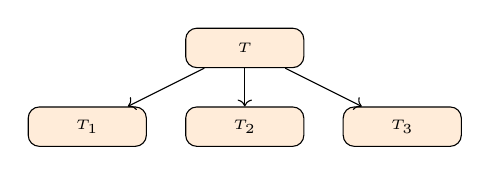
\begin{tikzpicture}
    \tikzset{emptydot/.style={fill=white,circle}}
    \tikzset{base/.style = {rectangle, rounded corners, draw=black,
                           minimum width=1.5cm, minimum height=0.5cm,
                           text centered, font=\sffamily\tiny}}
    \tikzset{action/.style = {base, fill=blue!30}}
    \tikzset{abstract/.style = {base, fill=orange!15}}

    \node (T) [abstract] at (5,2) {$T$};
    \node (T1) [abstract] at (3,1) {$T_1$};
    \node (T2) [abstract] at (5,1) {$T_2$};
    \node (T3) [abstract] at (7,1){$T_3$};

    \draw[->] (T) -- (T1);
    \draw[->] (T) -- (T2);
    \draw[->] (T) -- (T3);

\end{tikzpicture}
\end{center}\\
\vspace{-10pt}
\begin{center}
\textcolor{gray}{$T \rightarrow T_1, T_2, T_3 \; [T_1 \prec T_2 \prec T_3, between(T_1,p,T_3)]$}
\end{center}
\end{tabular}

\rule{\linewidth}{0.4pt}

\renewcommand{\arraystretch}{0.1}
\begin{tabular}{p{0.95\linewidth}}
\begin{center}
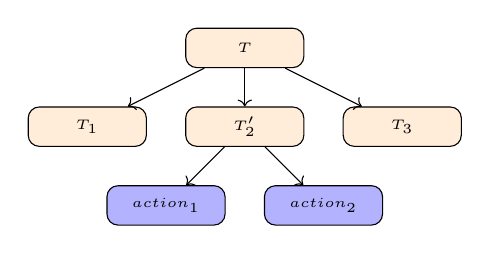
\begin{tikzpicture}
    \tikzset{emptydot/.style={fill=white,circle}}
    \tikzset{base/.style = {rectangle, rounded corners, draw=black,
                           minimum width=1.5cm, minimum height=0.5cm,
                           text centered, font=\sffamily\tiny}}
    \tikzset{action/.style = {base, fill=blue!30}}
    \tikzset{abstract/.style = {base, fill=orange!15}}

    \node (T) [abstract] at (5,2) {$T$};
    \node (T1) [abstract] at (3,1) {$T_1$};
    \node (T2) [abstract] at (5,1) {$T'_2$};
    \node (T3) [abstract] at (7,1){$T_3$};
    \node (act1) [action] at (4,0){$action_1$};
    \node (act2) [action] at (6,0){$action_2$};

    \draw[->] (T) -- (T1);
    \draw[->] (T) -- (T2);
    \draw[->] (T) -- (T3);
    \draw[->] (T2) -- (act1);
    \draw[->] (T2) -- (act2);

\end{tikzpicture}
\end{center}\\
\vspace{-10pt}
\begin{center}
\textcolor{gray}{$T \rightarrow T_1, T'_2, T_3 \; [T_1 \prec T'_2 \prec T_3]$; \\ $T'_2 \rightarrow action_1, action_2 \; [action_1 \prec action_2, be\text{f}ore(p, action_1), be\text{f}ore(p,action,2)]$}
\end{center}
\end{tabular}

\end{posterbox}

\begin{posterbox}[column=1, name=implementation, below=trans]{6. Implementation}

The practical part of this thesis aims to deliver some of the \emph{totally-ordered} transformations mentioned in the thesis. For this task, a user defines \emph{a hierarchical planning domain} using a simple text format and selects the desired transformation.

\vspace{5mm}

The program is written in C\# using the .NET8 framework and provides \emph{totally-ordered} transformations e.g. compile away all \emph{between-constraints} or \emph{empty methods}.

% \begin{itemize}
%     \item Remove all \emph{between-constraints} from \emph{the domain},
%     \item Remove all \emph{empty methods} from \emph{the domain},
%     \item Convert the input \emph{domain} in the one in HTN-ChNF.
% \end{itemize}

\end{posterbox}

\begin{posterbox}[column=1, name=conclusion, below=implementation, headerColorOne=green!59!yellow, boxColorOne=green!10]{7. Conclusions}

To conclude, this project consists of three main parts: \textbf{HTN Semantics}, \textbf{Transformations}, and an attached command-line \textbf{program}. Some transformations might be useful to achieve prerequisites for particular HTN planners, such as compiling away unsupported features. Other transformations (HTN-ChNF, -GNF) might speed up the \emph{planning} process and the reverse process of \emph{plan verification}.

\end{posterbox}

\begin{posterbox}[column=1, name=info, below=conclusion]{8. Additional Information}

\paragraph{Supervisor:} Prof. RNDr. Roman Barták, Ph.D.
\paragraph{Department:} Department of Theoretical Computer Science and Mathematical Logic
\paragraph{Thesis:} https://github.com/damodarak/bachelor-thesis

\end{posterbox}

\end{poster}
\end{document}